\chapter{Literature Review}

\begin{enumerate}
	\item [Technology] background 
	\item Depth Sensor technology + How Kinect works
	\item Point cloud map
	
	\item [Coding] references/Getting started
	\item Code references and and blog posts? 
	\item Previous example
	\item Hand Example
	
	\item [Mathematics] Used
	\item Papers on ellipse circumference
	
	\item [Improving] Accuracy
	\item Skeleton Joints filtering
	\item Error Model
	
	\item [Further] developments
	\item Augmented reality paper
	
	\item [Imaging] Processing Background
	\item Basics of an image - RGB
	\item Matlab
	\item Camera Model
	
	\item [Uncertainty] Measurements
	\item Gaussian 
	\item Triangular
\end{enumerate}

\hl{!!!!!!!!!!!!!!!!!!!!!Explain Lit Review Layout}\\

\section{Literature Guide}
\subsection{Getting Started}

\subsubsection{Non-Contact Human Body Parameter Measurement Based on Kinect Sensor \cite{nonContact2017}}

\paragraph{Overview}
This journal article provides an adequate base to understand many techniques used during this project. In the article, a similar project is explored in terms of using a Kinect to determine various personalized measurements. This includes measurements such as height, shoulder length, other key limb lengths and front perimeter measurements for the chest, stomach and waist. All of the work done in this article is similar to the work done in the initial stages of this project. The article also provides useful contextual information regarding the current use of this technology and background knowledge regarding the inner workings of the Kinect. 

\paragraph{Relevance}
The main contribution of this article was the background information it provided, together with the validation of certain aspects of the experiment methodology: 

\subparagraph{Background Theory}
This article provides a summary and overview of the process the Kinect utilises to retrieve data about a detected human. It explains the different sensors the Kinect posses, together with a basic understanding of the internal process required to track a skeleton and return information such as "Joint" position etc. This is explained in more detailed in Section \hl{(Reference to Middleware)}. It also provided an explanation of how pixels in the image plane are converted to real world positional points using information from both depth and colour frames. This is also explained in detail in Section \hl{(Depth - real conversion)}.

\subparagraph{Methodology}
This article was found after an initial strategy for calculating measurements was created. However, it served as a validation of the methods used, specifically with regards to using the Pythagorean Theorem in 3D space to calculate distances and for calculating the error between actual measurements and measurements obtained using the Kinect. These methods and the relevant equations are explained in Section \hl{(Measurement - Pyth + error)}. A method was also suggested for the calibration of results to improve their accuracy. However, this technique was not employed in this project. Reasons for the exclusion are given in Section \hl{(Design - No calibration or correction)}

\subsubsection{Real-Time Hands Detection in Depth Image by Using Distance with Kinect Camera \cite{handDetection2015}}

\paragraph{Overview}
This journal article explored various techniques to improve hand detection using a Kinect. The main focuses were in the areas of background removal, noise removal and feature extraction. Traditional image processing techniques require a large amount of processing power and often produced ambiguous results, with regards to feature extraction, and were prone to noise. Introduction of the Kinect allowed for the use of depth data to reduce the computational power needed and to improve the accuracy of the results. A large section of the paper was dedicated to "Shadow Removal", which is the process of removing depth data unavailable due to an object obstructing the emitted Infrared Rays. "Shadow" was determined to be a significant source of noise in the depth data and its removal improved the accuracy of the system.    

\paragraph{Relevance}
This article was very specific to the detection of hands and therefore its use was limited. However, valuable insights were gained regarding the "Shadow Removal" and Background Removal processes implemented \hl{(Classifier Maybe)}:

\subparagraph{Shadow Removal}
The intricacies of Kinect in creating a depth image using its IR Emitter and IR Camera were explored in more detail. This further expanded on the inner workings of the Kinect and contributed to Section \hl{(Depth Image Creation - Kinect)}. Additionally, this brought attention to a significant source of noise in the depth image and provided a method to improve the accuracy of measurement results. This method is explored in Section \hl{(Rec - Noise Removal)}

\subparagraph{Background Removal}
This article detailed a method of Background Removal that did not utilise the BackgroundRemoval API available in the Kinect for Windows SDK. This method provides an alternative method for background that could be investigated if the BackgroundRemoval API does not provide the desired results. This is explored further in Section \hl{(Rec - Background Removal)}

\subsubsection{A Real Time Virtual Dressing Room Application using Kinect \cite{virtualDress2012}}

\paragraph{Overview}
This report details and explains an approach used to create a virtual dressing room. The end result was an application that allowed a user to see what clothing would look like by augmenting it onto their body. This was executed in a three part process of user extraction, user tracking and clothing mapping. A Kinect sensor was used to extract the user from the background using depth images and user information. The Kinect was also used to track the skeleton of the user and create a coordinate system on which the virtual clothing could be mapped. Lastly, information including joint orientation and key body lengths were used to augment the clothing model onto the body.  

\paragraph{Relevance}
This report details and explains a possible extension on this project that would be very useful in a production level solution. 

\subparagraph{Augmented Reality}
The virtual dressing room proposed in the report is foundational solution using augmented reality and requires further work and research in itself. However, once it is improved to a level sufficient for implementation, it would significantly improve the customer experience. This is envisioned to be used after the customer uses the system, proposed in this report, to determine their full body parameters. The customer would be able to use the virtual dressing room to get an accurate understanding of how different clothes would look on them, without needing to physically try them on. This is expanded on in Section\hl{(Rec - Virtual Dressing Room)} 

\subsubsection{Performance Evaluation of the 1st and 2nd Generation Kinect For Multimedia Applications \cite{kinectComp2011}}

\paragraph{Overview}
This report evaluates the performance of the Xbox 360 Kinect (First Generation - v1) and the Xbox One Kinect (Second Generation - v2). The launch of the Kinect v1 in 2010 was revolutionary as it made depth acquisition more affordable and accessible to a wide spectrum of users. Further excitement was created when Microsoft launched the Kinect v2 only three years later. However, the technology used for depth acquisition in the second generation Kinect was completely different to that of the first. The first generation Kinect utilised structured light which is a well known technology used by industry grade laser scanners for 3D construction. The second generation Kinect, on the other hand, uses a Time-Of-Flight (ToF) camera. This drastic changed piqued interest about the performance difference between the sensors and their ideal applications. Consequently, this report is among many written to quantify the difference. 

\paragraph{Relevance}
This report provided in depth knowledge about the principle of operation of the Kinect used in this project, together with its successor. This information contributed both to the background theory for the Kinect's operation and to component selection.

\subparagraph{Background Theory}
The first generation Kinect which is utilised in this project, operates on a principle known as structured light. This knowledge is provides an essential base of understanding that allows for the effect manipulation of data retrieved from the sensor. Also, it provides more information regarding the limitations of the technology. As such, ideal operating conditions can be determined which greatly aids in experimental design. More detail is given in Section \hl{(Sensor Background)}.

\subparagraph{Component Selection}
This report aided in the selection of a component for the design. The results yielded that the second generation Kinect on average performs better than the first generation Kinect. However, a large amount of performance testing was done in extreme conditions such as in direct sunlight, in darkness, at far distances etc. Consequently, significant disparity in the performance occurred mostly in these special conditions. For the purposes and operating conditions of the project, the first generation Kinect is sufficient. Elaboration into the evaluation between the two sensors is done in Section \hl{Component Selection} 

\subsubsection{Kinect for Windows Sensor Components and Specifications \cite{msdnKinectSpecs2017}}

\paragraph{Overview}
This technical documentation provided by Microsoft details the components that comprise the Kinect sensor and its specifications. This provides background information regarding the types of information it provides and a high-level description of how the sensor operates.

\paragraph{Relevance}
This high-level description of the Kinect provides the foundation of background information that is required before development with the Kinect can take place. 

\subparagraph{Background Theory}
The essential information retrieved from this document include a description of each component segment of the Kinect and their respective specifications. The key details retrieved are as follows: 
\begin{itemize}
	\item The resolution of the RGB camera
	\item The operation of the depth sensor
	\item Frame rates for the depth and colour stream
	\item Viewing angle or field of view of the Kinect
	\item Vertical tilt range
	\item The accelerometer used to detect to determine the orientation of the Kinect 
\end{itemize}

\subsubsection{Depth Camera \cite{msdnDepthCamKinect2017}}

\paragraph{Overview}
This technical documentation provided by Microsoft Robotics details more specific operations and interfaces to interact with the depth camera. This is a generic document for all depth camera devices that are supported by Microsoft.  

\paragraph{Relevance}
This document does not provide specific information regarding how to interact with the Kinect's API to interface with the depth sensor and manipulate depth data. However, it provides essential information regarding how depth data is stored in all Microsoft devices with this functionality. 

\subparagraph{Background Theory}
The key details extracted from this document that inform the use of depth data retrieved from the Kinect are as follows: 
\begin{itemize}
	\item A brief introduction to the depth image space.
	\item The information stored in depth data.
	\item The bit size of the depth data and the relevance of each bit.
\end{itemize}

\subsubsection{Coordinate Spaces \cite{msdnCoSpaces2017}}

\paragraph{Overview}
This technical documentation provided by Microsoft details the coordinate spaces for the three streams of data available - Colour, Depth and Skeleton. This provides background information explains how to interpret the data explains the manner in which it is stored. It also provides a brief introduction to how to use the API to transform data between the different spaces.

\paragraph{Relevance}
This description expands on the introductory theory provided on the component composition of the Kinect. This forms the reference used for digital representation of real world information captured by the relevant sensing components. It delves deeper into the intricacies of each of the data types and provides the base for interpreting and manipulating the data algorithmically. The detailed explanation of this information is included in Section \hl{(Coordinate Spaces Ref)}. A brief expansion on the most significant information utilised from this document is seen below: 

\subparagraph{Colour Space}
All the real world data available in the field of view of the RGB camera is captured and available as a frame of data. The frame is made of a number of pixels depending on the resolution specified. Each pixel at a particular (x, y) coordinate on the colour frame contain values for red, green and blue colour.

\subparagraph{Depth Space}
A depth frame is available that is a grayscale representation of everything in the field of view of the camera. Like the Colour Space, the frame consists of a number of pixels depending on the resolution. However, these pixels hold the distance of the nearest object in millimetres at a given (x, y) coordinate. The (x, y) coordinate correspond to the position of the pixel on the depth frame and have no direct correlation with dimensions in physical space.
	
\subparagraph{Skeleton Space}
Depth image data is processed to produce a frame of skeleton data. All points in skeleton space are in 3D. The Kinect acts as the point of origin with a positive x-axis extending to the left, a positive y-axis extending upwards and a positive z-axis extending in the direction the Kinect is pointing. Skeleton data can also be used to track human skeletons and provide positional data of the skeleton.

\subsubsection{Skeletal Tracking \cite{msdnSkelTrack2017}}

\paragraph{Overview}
This technical documentation provided by Microsoft explains the high-level functioning of the Kinect's skeletal tracking capabilities. It provides an overview of how the Kinect recognises people and various operating conditions for effective tracking.

\paragraph{Relevance}
Understanding how the skeletal tracking system operates is essential in understanding the strengths and weaknesses of using the Kinect for human body detection. Additionally, the information regarding operating conditions advises various aspects of the experiment design procedure. 

\subparagraph{Background Theory}
The skeletal tracking capability is a complex and multifaceted system. Before it can be successfully incorporated into another system or application, it is vital to obtain thorough knowledge of each level of functionality and operation. This document provides the starting point for this journey as it provides a condensation of the capability. More detail is given in Section \hl{(Skeletal Tracking - Ref)}

\subparagraph{Design}
This document also provides important insights into the operating conditions required for skeletal tracking. These are refereed to when designing the experiment and overall solution in Sections \hl{(Insert 2 refs to skeletal conditions)}. Examples of these operating conditions are listed below:
\begin{itemize}
	\item The orientations of the human body for which the Kinect operates successfully as well as those with which it falters.  
	\item The field of view restrictions of the Kinect
\end{itemize}

\subsubsection{Tracking Users with Kinect Skeletal Tracking \cite{msdnTrackUserSkel2017}} \label{litTrackSkelUsers}

\paragraph{Overview}
This technical document provided by Microsoft provides a comprehensive walk-through and explanation on how to use the Kinect API to access skeletal information. It provides C++ and C\# code snippets to successfully enable user tracking, identify user skeletons and access positional information.

\paragraph{Relevance}
The skeleton tracking capability of the Kinect forms the major foundation of this project. This document provides information that makes navigating the API seamless and provides foundational understanding for unpacking code samples available by Microsoft. It is therefore a crucial piece of information to familiarise oneself with the Kinect API before application development can commence. 

\subparagraph{Background Theory}
The skeletal information provided by the Kinect API is intuitive to understand and utilise. However, there are important nuances that must be understood to prevent unwanted errors during development. These details are discussed thoroughly in Section \hl{(Insert Skeletal Ref - Joint states etc.)}. 

\subparagraph{Design}
This document proved critical in algorithm design of the solution. The nature of certain API interactions advised certain decisions regarding the application's class architecture and integration with other parts of the solution. Further explanations are given in Section \hl{(Algorithm Design - Skel Tracking)}. 

\subsubsection{Formula Derived Mathematically for Computation of Perimeter of Ellipse \cite{ellipsePerimeter2012}}

\paragraph{Overview}
The ellipse is a widely used shape that forms a crucial part of mathematics. Some of its uses include, but are not limited to, conic sections and Keplar's law od Planetary Motion. Despite, its prevalence in many applications, there does not exist a set formula that allows the perimeter to be calculated from the axes of the ellipse. Instead, all methods used to date for calculation, are approximations. This journal article, explores these existing methods, proposes a new formula that relates the radius to the perimeter and evaluates their performances.The proposed method performed very close to or better than many existing models. As such, the formula relationship can be utilised and allows for efficient perimeter determination using the major and minor axes.

\paragraph{Relevance}
The second major part of this project is the modelling of 3D circumferences using measurements obtained by the system. A model to determine these circumferences must be developed and as such, various mathematical shapes or parametric models should be tested. The ellipse is one such shape. 

\subparagraph{Design}
It is theorised in this project that a body part can be modelled within a certain error margin using the ellipse as a model. As such, the formula proposed in this article was utilised forms a fundamental part of the modelling stage of the algorithm. This is expanded on in Section \hl{(Ellipse Ref - Design)}.

Programming Guide + Documentation\\
Uncertainty\\
Clothing\\

Definitions!!!!!!!!!!!!!!!!!\\
Accuracy\\
Precision\\
Kinect\\
Volunteer\\
Operator\\
IR - Infrared Rays\\
API\\
RGB\\
SDK\\


When writing your review start of with the general concepts and move to the more specific aspects
explaining the necessary theory as you go. This section is NOT a copy and paste from others work or a
rewrite-but-change-one-word section. I suggest you read all your material, and then put it down and
write this section, referring back to the work only when you need to check something.

See your PCS textbook for more details on how to write a literature review.

If you include a figure or a table in your text please see the example in Fig. \ref{fig:model} as to how to caption it.
Please make sure that all text in your figures is readable and that you reference your figures if they are
from another source.

\begin{figure}[ht]
\centering
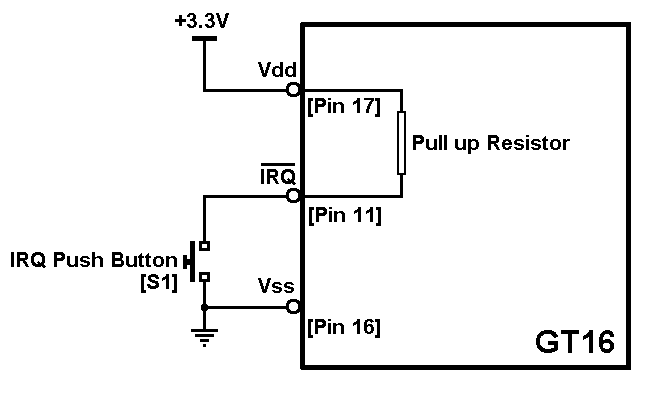
\includegraphics[width=0.7\textwidth]{model.png}
\caption{A block diagram illustrating the connections to the IRQ pin on the MCS08GT16A microcontroller (Please
note that your headings should be short descriptions of what is in the diagram not simply the figure title)}
\label{fig:model}
\end{figure}

